% !TeX spellcheck = de_DE
\documentclass[a4paper, 12pt]{article}

\usepackage{bm, bbm, wrapfig, float, setspace, amsmath, amssymb, amsthm, url, graphicx, ngerman, transparent, enumerate, bbold, esint, polynom, hyperref, microtype, etoolbox, braket, cleveref, hyphenat, stmaryrd}
\usepackage{centernot}

\usepackage{tikz}
\usepackage{epsdice}
\usepackage{listings}
\lstset{language=Python}
\tikzset{>=stealth}
\usetikzlibrary{decorations.markings, shapes, calc}

\renewcommand{\familydefault}{cmss}   % Generates sans serif fonts


\renewcommand{\l}{\left(}
\renewcommand{\r}{\right)}
\newcommand{\gs}{\text{gs}}
\renewcommand{\P}{\hat{P}}
\newcommand{\U}{\hat{U}}

% \newcommand{\bra}[1]{\langle#1|}
% \newcommand{\ket}[1]{|#1\rangle}
\newcommand{\bkt}[2]{\left\langle #1 |#2 \right\rangle}
\renewcommand{\ij}{{\langle \vec{i}, \vec{j} \rangle}}
\renewcommand{\H}{\hat{\mathcal{H}}}
\newcommand{\Ht}{\tilde{\mathcal{H}}}
\renewcommand{\c}{\hat{c}}
\renewcommand{\a}{\hat{a}}
\newcommand{\cd}{\hat{c}^\dagger}
\newcommand{\rh}{\hat{\rho}}
\newcommand{\rht}{\tilde{\rho}}
\newcommand{\ad}{\hat{a}^\dagger}
\newcommand{\bd}{\hat{b}^\dagger}
\newcommand{\ubd}{\hat{\uline{b}}^\dagger}
\newcommand{\ub}{\hat{\uline{b}}}
\renewcommand{\b}{\hat{b}}
\newcommand{\hd}{\hat{h}^\dagger}
\newcommand{\h}{\hat{h}}
\renewcommand{\d}{\hat{d}}
\newcommand{\n}{\hat{n}}
\newcommand{\D}{\hat{D}}
\newcommand{\Dd}{\hat{D}^\dagger~\hspace{-0.12cm}}

\newcommand{\G}{\hat{\Gamma}}
\newcommand{\Gd}{\hat{\Gamma}^\dagger}
\newcommand{\F}{\hat{F}}
\newcommand{\Fd}{\hat{F}^\dagger}
\newcommand{\hc}{\text{h.c.}}
\newcommand{\MF}{\text{MF}}
\newcommand{\BEC}{\text{BEC}}
\newcommand{\RG}{\text{RG}}
\newcommand{\psd}{\hat{\psi}^\dagger}
\newcommand{\ps}{\hat{\psi}}
\newcommand{\I}{\text{I}}
\newcommand{\p}{\text{p}}
\newcommand{\f}{\text{F}}
\newcommand{\s}{\text{S}}
\renewcommand{\sf}{\text{MIX}}
\renewcommand{\O}{\hat{\mathcal{O}}}
\newcommand{\W}{\hat{W}}
\newcommand{\Ud}{\hat{U}^\dagger}
\newcommand{\HMF}{\mathscr{H}_{\text{MF}}}
\newcommand{\ph}{\text{ph}}
\newcommand{\IB}{\text{IB}}
\newcommand{\B}{\text{B}}
\newcommand{\eff}{\text{eff}}
\newcommand{\tr}{\text{tr}}
\newcommand{\tdiff}{\,\mathrm{d}}
\newcommand{\nodagger}{{\vphantom{\dagger}}}
 % \newcommand{\longmapsfrom}{\longleftarrow\!\shortmid}

\normalsize
\setlength{\hoffset}{-1.5cm}
\addtolength{\textwidth}{3cm}
\setlength{\voffset}{-2.2cm}
\addtolength{\textheight}{3.5cm}
\addtolength{\footskip}{0.2cm}

%\input{macros.tex}
\newtheorem{aufgabe}{Problem}
\newtheorem{bspaufgabe}{Beispielaufgabe}

\usepackage{titlesec}

\titleformat{\section}[block]
{\normalfont}{\textbf{Problem \thesection}}{1em}{}

\DeclareMathOperator{\dd}{d}
\newcommand{\eul}{\text{e}}

% imaginary unit 
\newcommand{\imag}{\textsl{i}}
%
% with or without solution?
%
\makeatletter
\@ifundefined{solfalse}{
\newif\ifsol
\soltrue
}
\makeatother
\newcommand{\solA}{\vskip0.5em \color{brown}\noindent\textbf{Solution:\\}}
\newcommand{\sol}[1]{\vskip0.5em \color{brown}\noindent\textbf{Solution:}\\#1}

\usepackage{relsize}
\newcommand\Cpp{C\nolinebreak[4]\hspace{-.05em}\raisebox{.4ex}{\relsize{-3}{\textbf{++}}}}

\begin{document}
	   
% ********** First Box **************
\vspace*{-13mm}
\noindent\fbox{
	\parbox[b][19mm][b]{16mm}{%\parbox[POS][H�HE][POS-INNEN]{BREITE}{INHALT}
		\center
\includegraphics[trim=1.6mm  0 0 0, width=18mm]{../../images/lmu-bildmarke.png}
	}
}
\hfill
% ********** Second Box **************
% Diese Schrift sollte so gross sein, dass die Oberkante des Ms von
% Max mit der Oberkante von LMU abschliesst
\fbox{\parbox[b][19mm][b]{19mm}{
\includegraphics[width=19mm,height=19mm]{../../images/lmu-wortmarke.png}}}%
\hfill\hfill
% ********** Third Box **************
\fbox{\parbox[b][19mm][b]{84mm}{\fontsize{9}{12}\sc Faculty of Physics, Summer Term 2023 \\  Numerical Quantum Physics\\ 
		Lecturer: Dr. S. Paeckel \\ Assistant Lecturer: Z. Xie, B. Schneider
		\vspace{0.1mm}}}
\hfill
% ********** Fourth Box **************
\fbox{
	\parbox[b][19mm][b]{25mm}{\hspace*{3mm}\transparent{0.52}{\vspace{-1mm}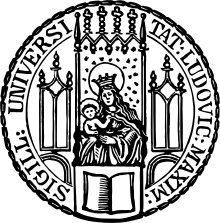
\includegraphics[trim=0 6mm 16mm 20mm, clip, height=21mm]{../../images/lmu-siegel.png}}\transparent{1}}
}
\begin{center}
	\small \url{https://www2.physik.uni-muenchen.de/lehre/vorlesungen/sose_23/nqp/}
\end{center}
%
\vspace{8mm}
%
\centerline{\Large\textbf{Sheet~4:~Quantum Monte-Carlo}}
%
\vspace{3mm}
%
\normalsize\centerline{Released:~06/09/23;~Submit until:~06/23/23 (\textbf{20 Points})}
%
%\vspace{0mm}
%
%
\vspace{6mm}
%
On this sheet we realize an efficient, yet conceptionally simple, Monte-Carlo sampling to generate configurations of spin-$1/2$ degrees of freedom, distributed according to the Boltzmann statistics, using \textit{cluster algorithms}.
%
We will consider the Ising model on a square lattice in $d=2$ dimensions with $L^2$ lattice sites ($L\in\mathbb N$):
\begin{equation}
	\hat H = -J \sum_{\braket{i,j}} \hat Z_i \hat Z_j
\end{equation}
and choose as computational basis the Pauli $\hat Z$-operator eigenstates $\ket{\sigma_j}$ with $\sigma_j \in \left\{+1, -1 \right\} \equiv \mathcal S$.
%
The goal is now to draw samples of configurations $\underline C \in \mathcal S^{L^2}$ that are distributed according to the Boltzmann distribution $p(\underline C) = \mathrm{e}^{-\beta E[\underline C]}/Z_\beta$ at an inverse temperature $\beta = 1/T$ and $E[\underline C]$ denotes the energy of the configuration $\underline C$.
%
Once this is achieved, we can estimate observables (here functions of Pauli $\hat Z$-operators) by calculating expectation values with respect to a set of generated samples $\mathcal C \subset S^{L^2}$:
\begin{equation}
	\braket{\hat A} \approx \bar A = \frac{1}{\lvert \mathcal C \rvert} \sum_{\underline C \in \mathcal C} A[\underline C] \; .
\end{equation}
%
\section{A Markov chain for cluster updates \textbf{(14 Points)}}
%
In cluster algorithms, the partition function $Z=\operatorname{Tr} \mathrm{e}^{-\beta \hat H}$ is further expanded in a set of graphs $\mathcal G$, i.e., equal-time slices through world lines, that belong to the same configuration $\underline C$.
%
Here, a world line is given by the evolution of an initial configuration $\underline C_0$
\begin{equation}
	\ket{\underline C_0} \stackrel{p(\underline C_1|\underline C_0)}{\longrightarrow} \ket{\underline C_1} \stackrel{p(\underline C_2|\underline C_1)}{\longrightarrow} \cdots \stackrel{p(\underline C_M|\underline C_{M-1})}{\longrightarrow} \ket{\underline C_M} \; ,
\end{equation}
with $M\in\mathbb N$, which constitutes a Markov process.
%
For a certain configuration and compatible graph $(\underline C_n, G_n)$, it is realized by performing a graph update with probability $p(\underline C_n, G_{n+1} | G_{n})$, followed by an update of the configuration, compatible with the new graph, with probability $p(\underline C_{n+1}|\underline C_n, G_{n+1})$.
%

%
For the Ising model, this process can be obtained by noting that only neighboring spin can be flipped and there are two possible graphs associated.
%
If under a transition $\underline C_n \longrightarrow \underline C_{n+1}$ a pair of spins is to be flipped, we denote the corresponding graph to be connected, otherwise the graph is called disconnected.
%
\begin{itemize}
	\item[(1.a)] \textbf{(3P)}
	%
	Implement a lattice class which hosts a configuration $\underline C$ of spin-$1/2$ degrees of freedom on a two-dimensional lattice with dimensions $L \times L$.
	%
	Equip the class with a method to compute the average magnetization $m=\braket{\hat Z}$.
	%
	Furthermore, implement a method that initializes the lattice with a random configuration of spin.
	%
	\item[(1.b)] \textbf{(3P)}
	%
	Implement an update class that acts as base class for a cluster update.
	%
	It should provide an abstract method that takes as input a configuration $\underline C$ and returns a new configuration $\underline C^\prime$.
	%
	Extend your lattice class by an \texttt{update} method that takes as input argument an instance of the update class (updater) as well a number of updates $N_u$ to be performed and which then calls the updater $N_u$ times to generate a new lattice configuration.
	%
	\item[(1.c)] \textbf{(4P)}
	%
	Derive from the basic update class to implement the Swendsen-Wang algorithm.
	%
	Here, an update is defined by
	\begin{itemize}
		\item To each neighboring pair of parallel aligned spins in the lattice, assign with probability $1-\mathrm{e}^{-2\beta J}$ a label \textit{connected} or label it as \textit{disconnected}.
		%
		\item Find all clusters of connected spins.
		%
		\item The spins in each cluster are flipped with probability $1/2$.
		%
	\end{itemize}
	%
	\item[(1.d)] \textbf{(4P)}
	%
	Derive from the basic update class to implement the Wolff algorithm.
	%
	Here, an update is defined by
	\begin{itemize}
		\item Choose a random spin as initial cluster.
		%
		\item Label all neighboring spins that are parallel to the initial spin as \textit{connected} with probability $1-\mathrm{e}^{-2\beta J}$.
		%
		\item Repeat the previous step for all spins that have been newly added to the cluster recursively, until the cluster is not growing any more.
		%
		\item Flip all spins in the cluster.
		%
	\end{itemize}
	%
\end{itemize}
%

%
\section{Autocorrelation times \textbf{(6 Points)}}
%
We now test the different cluster update methods by computing the autocorrelation times.
%
These are crucial to ensure that the configurations generated by one update run can be considered to be independent, i.e., they constitute independent samples, drawn from the jont probability distribution $p(\underline C)$.
%
Deviations of the sample independence affect the estimation of expectation values $\bar A$ of observables via the autocorrelation $c_A(t)$:
\begin{equation}
	\operatorname{Var}[\bar A] = \frac{\operatorname{Var}[\braket{\hat A}]}{N_\mathcal{C}} \left(1 + 2\sum_{t=1}^{N_\mathcal{C}-1}(1-\frac{t}{N})\frac{c_A(t)}{c_A(0)})\right)
\end{equation}
with $N_\mathcal{C} = \lvert \mathcal C \rvert$.
%
The autocorrelation is defined via
\begin{equation}
	c_A(t) = \braket{A_0 A_t} - \braket{A}^2 \;,
\end{equation}
where $\braket{A_0 A_t}$ denotes the expectation value w.r.t. to the $0$th and $t$th samples of the $N_\mathcal{C}$ realizations.
%
\begin{itemize}
	\item[(2.a)] \textbf{(3P)}
	%
	For both update methods implemented, run $N=100$ Monte-Carlo simulations at inverse temperatures $\beta=0.1,\ldots,10.0$ (with a proper discretization for the $\beta$'s), choosing $N_u=100$ Markov steps and $N_\mathcal{C}=50$ configurations per simulation.
	%
	Start each simulation from a random configuration and use $N_u$ initial updates to erase the memory of the initial state (burn-in).
	%
	In every simulation after each cluster update, measure the cluster's magnetizations $m$ and store the sequence of $N_\mathcal{C}$ measurement results.
	%
	\item[(2.a)] \textbf{(3P)}
	%
	Compute the autocorrelation $c_m(t)$ for both update schemes.
	%
	Estimate the integrated autocorrelation time $\tau_m = \sum_{t=1}^{N_\mathcal{C}-1}(1-\frac{t}{N})\frac{c_m(t)}{c_m(0)})$ and compare it to the sample variance of the magnetization.
	%
\end{itemize}
%
\batchmode  % This suppresses some verbose LaTeX output
\end{document}

